\subsection{La recherche bibliographique}
Avant d'espérer pouvoir commencer le développement de l'outils, mon maître de stage, Laurent Lefèvre, m'a conseillé de commencer par une grande recherche bibliographique afin d'intégrer les problématiques de Green IT et plus particulièrement de chercher des indicateurs qui pourraient nous intéresser pour mesurer l'empreinte environnementale des centres de données. Je me suis tout d'abord intéresser aux indicateurs fournis par l'organisme GreenGrid qui fut le premier à fournir ce genre d'indicateur de Green IT pour les centres de données.\\

Dans cette partie nous présenterons et critiquerons l'ensemble des indicateurs que j'ai retenu pour les intégrer dans le simulateur.

\subsubsection{Power Usage Effectiveness (PUE)}
Les centres de données effectuent de nombreuses dépenses énergétiques pour placer le matériel informatique dans des conditions optimales de fonctionnement : refroidissement de l'air, stabilité et qualité de l'électricité, sécurité du bâtiment etc. Il est alors intéressant de comparer la part d'énergie utilisée pour ces dépenses auxiliaires et la part allouée au \gls{travailutile} du data-centre.\\

Le PUE est un indicateur créé par l'organisme GreenGrid qui montre la part d'énergie utilisée par tout ce qui entoure le matériel informatique par rapport à la part utilisée par le matériel informatique lui-même. Il est défini par la formule suivante :

\[PUE=\frac{Consommation\ de\ l'\acute{e}tablissement}{Consommation\ de\ l'\acute{e}quipement\ informatique}\]\\
Ainsi un PUE de 3 indique que le centre de données utilise 3 fois plus d'énergie en infrastructure qu'en travail utile. Il existe également une variante du PUE sous forme d'indice, appelé DCE et calculé comme l'inverse du PUE, il permet d'obtenir une valeur bornée entre 0 et 1.\\

Le PUE s'est imposé durant les dernières années comme norme afin de comparer l'efficacité énergétique des data-centre et est même considéré par certains comme un critère \og éco-responsable \fg{}. Pour plus de simplicité on a alors découpé le PUE en 7 classes énergétiques :

\begin{figure}[h]
	\begin{center}
		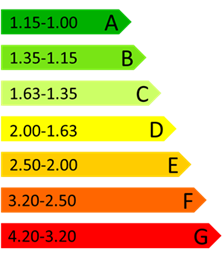
\includegraphics[scale=0.6]{partie2/images/classeEnergetique.png}
	\end{center}
	\caption{Les classes énergétiques du PUE}
\end{figure}
\newpage
Cependant, il ne faudrait pas lui donner des propriétés qu'il ne possède pas. Malgré la tendance actuelle accommodée au green-washing, le PUE n'est pas très bien choisi pour comparer des data-centres entre eux. Des éléments manquent pour une comparaison juste et efficace : localisation géographique, taux de disponibilité ou taux de charge \cite{badPUEOtherMetrics}. De plus, le mode de calcul possède un biais : baisser la quantité d'énergie utilisée par l'équipement informatique, même si c'est pour une meilleur gestion de l'énergie fait augmenter le PUE. La virtualisation par exemple fait augmenter le PUE alors qu'elle offre une puissance de calcul par unité d'énergie plus importante \cite{badPUEVirtualisation}. Le même raisonnement peut être appliqué à la gestion de la charge, qui, en éteignant certains équipements informatiques, fait augmenter le PUE \cite{badPUECharge}.\\

Cependant, s'il on prend le PUE comme il est, c'est à dire un indicateur qui montre la proportion d'énergie utilisé par l'architecture du centre de données par rapport à la consommation de l'équipement informatique et non pas un fer-de-lance de l'éco-conception des centres de données il reste pertinent pour notre simulateur.

\subsubsection{Carbon Usage Effectiveness (CUE)}
Cet indicateur est le deuxième indicateur de la famille xUE de l'organisme GreenGrid et aspire à devenir un standard dans l'industrie pour comparer les data-centres sur leurs rejets de dioxyde de carbone comme l'a été le PUE pour l'efficacité énergétique.

\[CUE=CEF \times PUE\]

Le CEF représente le facteur d'émission de dioxyde de carbonne pour un kWh, en France cette valeur vaut en moyenne \SI[per-mode = symbol]{74}{\g\per\kWh} \cite{co2PerkWh}. Cependant cette valeur moyenne n'est pas très précise, en effet on peut imaginer que des centre de données utilise certains fournisseurs d'énergie afin de limiter leur émissions de CO2, ou produisent leur propre énergie sur site. Afin d'obtenir une valeur correcte du CUE il faudra donc calculer le CEF en fonction de la quantité de gaz à effet de serre émise par chaque source d'énergie qu'utilise le centre de données.\\

Le CUE permet d'évaluer la quantité de CO2 produite par le data-centre en fonction de sa consommation d'énergie. La valeur optimale du CUE est donc zéro.

\subsubsection{Data Center energy Productivity (DCeP)}
\[DCeP=\frac{Travail\ utile}{Consommation\ de\  l'\acute{e}tablissement}\]\\
Le DCeP représente l'énergie nécessaire pour une opération. L'unité du \gls{travailutile} est à définir selon l'usage de l'indicateur, on peut imaginer un \gls{flop}, une exécution d'un programme, un client, une commande etc.\\

Grâce à cet indicateur on peut également évaluer la quantité de gaz à effet de serre rejetée dans l'atmosphère par unité de \gls{travailutile} en utilisant le facteur d'émission de dioxyde de carbone par kWh du centre de données ($CEF$).
\[CEF \times DCeP\]

Pour notre simulateur cet indicateur est difficile à exploiter car il est très difficile d'estimer la valeur du travail utile car c'est extrêmement spécifique. Cependant, il serait cependant dommage de ne pas donner la possibilité à l'utilisateur de le calculer si il en connait les détails.

\subsubsection{Green Energy Coefficient (GEC)}
\[GEC=\frac{Consommation\ \acute{e}nergie\ verte}{Consommation\ totale\ d'\acute{e}nergie}\]\\
Le GEC quantifie la part d'énergie renouvelable consommée par le data-centre. Ce coefficient permet de nuancer l'impact carbone du data-centre s'il utilise des énergies renouvelables.
La consommation d'énergie verte ne correspond pas à la part d'énergie renouvelable injectée dans le réseau électrique du fournisseur d'énergie, la data-centre doit posséder, ou posséder les droits d'utilisation, de cette source d'énergie.

\subsubsection{Energy Reuse Factor (ERF)}
\[ERF=\frac{\acute{E}nergie\ r\acute{e}utilis\acute{e}e\ \grave{a}\ l'ext\acute{e}rieur}{Consommation\ totale\ d'\acute{e}nergie}\]\\
Le ERF quantifie la quantité d'énergie réutilisée à l'extérieur du data-centre. Cette énergie peut prendre différentes formes : chaleur servant de chauffage, électricité résiduelle, mouvement etc. et est mesurée à la sortie du data-centre et convertie en kWh . Le but de cet indicateur est d'inciter les data-centres à réutiliser leur énergie résiduelle plutôt que la rejeter.

\subsubsection{Efficacité énergétique de l'équipement (EEE)}
Le Standard Performance Evaluation Corporation (SPEC) est un consortium proposant, entre autre, des \gls{benchmark} du matériel informatique. Son indicateur \emph{ssj\_ops} représente le débit de calcul (le nombre d'opération par seconde) durant un \gls{benchmark} effectué sous une machine virtuelle \gls{java} \cite{SPECpowerssj2008field}.\\

Le SPEC met également à disposition les mesures de consommation d'énergie pendant le \gls{benchmark} ce qui lui permet de déduire l'efficacité énergétique de l'équipement en calculant son nombre d'opérations par unité d'énergie consommée (\emph{ssj\_ops\_perwatt}). Le jeu de données contient 551 modèles de serveur commercialisés entre 2008 et 2018 \cite{SPECpowerssj2008}.\\

On peut alors définir l'efficacité énergétique de l'équipement du data-centre par la moyenne de l'efficacité de chaque équipement :

\[EEE_{DC}=\frac{1}{n}\sum_{i=1}^{n}{ssj\_ops\_perwatt}_i\]

Même si cette initiative nous permet d'avoir un ordre d'idée de l'efficacité énergétique de l'équipement, nous devons garder à l'esprit que les mesures, envoyées par de multiples organismes, ne sont pas vérifiées par le SPEC et qu'elle sont effectuées sous un environnement JAVA qui n'est pas forcement représentatif de l'utilisation d'un serveur de centre de données.

\subsubsection{KPI Global DCEM}
Ce meta-indicateur normalisée par l'Europe \cite{KPIDCEM} en réponse aux critiques à l'égard du PUE américain permet le suivi de la gestion énergétique d'un data-centre. Il est défini par 4 indicateurs que nous allons présenter qui permettent une interprétation plus fine des résultats.\\

Ce meta-indicateur se présente sous la forme d'un couple de valeur défini par $(DC_G, DC_P)$, représentant respectivement la taille du data-centre ainsi que sa classe énergétique.\\

\textbf{KPI Energy Consumption ($KPI_{EC}$)}\\
Cet indicateur représente l'énergie nécessaire pour le fonctionnement du data-centre pendant une année. Il prend en compte les dépenses énergétiques liées à l'infrastructure technique mais également celles liées à l'exploitation du data-centre : sécurité, gardiens, maintenance etc. Cependant il ne prend pas en compte la consommation d'énergie des bâtiments contenant les bureaux des employés qui mettent en place et utilisent le data-centre : chefs de projets, devOps etc.\\

Cet indicateur est très normalisé et détaillé dans son calcul, vous retrouverez en \hyperref[appendix:kpiec]{Annexe A} le calcul exact du $KPI_{EC}$.\\

\textbf{KPI Task Efficiency ($KPI_{TE}$)}\\
Cet indicateur représente le rapport entre la consommation d'énergie de tous les composants quels qu'ils soient ($EC_{DC}$) et celle des composants qui calculent, stockent ou transporte des données ($EC_{HE}$).
Tous les composants transformant l'électricité ou améliorant la disponibilité doivent être pris en compte ainsi que tous les équipements en aval des sources d'énergie : éclairage, climatisation, sécurité, distribution électrique, extraction de la chaleur etc.

\[KPI_{TE} = \frac{EC_{DC}}{EC_{HE}}\]

Cet indicateur rappelle le PUE à la différence qu'il est beaucoup plus précis dans la liste des équipements à prendre en compte, la méthode de mesure (à l'extérieur du composant et au plus près de son entrée et de sa sortie pour ne pas prendre en compte les pertes.\\

\textbf{KPI Energy Reuse ($KPI_{REUSE}$)}\\
Cet indicateur représente le rapport entre l'énergie réutilisée en dehors des équipements informatiques du data-centre ($EC_{REUSE}$) et l'énergie totale dépensée par le data-centre ($EC_{DC}$).
Voici les initiatives courantes pour la réutilisation de l'énergie :
\begin{itemize}
	\item La production d'eau chaude,
	\item Le chauffage des bureaux ou d'appartements adjacents,
	\item Le préchauffage des diesels
\end{itemize}

\[KPI_{REUSE} = \frac{EC_{REUSE}}{EC_{DC}}\]\\

\textbf{Datacenter Energy Consumption Gauge ($DC_G$)}\\
Cet indicateur définis le gabarit de consommation d'énergie du data-centre. Il est défini par le tableau suivant :

\begin{table}[h]
	\begin{center}
		\setlength{\tabcolsep}{2em}
		\def\arraystretch{1.25}
		\begin{tabular}{|c|c|}
			\hline
			$DC_G$ & Intervalle du $KPI_{EC}$ \\
			\hline
			S & $KPI_{EC} \leq \SI{1}{\giga\watthour}$ \\
			\hline
			M &  $\SI{1}{\giga\watthour} < KPI_{EC} \leq \SI{4}{\giga\watthour}$ \\
			\hline
			L & $\SI{4}{\giga\watthour} < KPI_{EC} \leq \SI{20}{\giga\watthour}$ \\
			\hline
			XL & $KPI_{EC} > \SI{20}{\giga\watthour}$\\
			\hline
		\end{tabular}
		\caption{Calcul du Datacenter Energy Consumption Gauge ($DC_G$)}
	\end{center}
\end{table}

\textbf{Datacenter Performance ($DC_P$)}\\
Cet indicateur défini la performance énergétique du data-center, il est obtenu par la formule suivante :

\[DC_P = KPI_{TE} \times (1 - W_{REUSE} \times KPI_{REUSE}) \times (1 - W_{REN} \times KPI_{REN})\]

$W_{REUSE}$ et $W_{REN}$ sont deux facteurs de modération susceptibles de changer en fonction de la taille du data-center, leurs valeurs par défaut sont 0,5. \\

Une fois calculé on pourra définir la classe à partir du tableau suivant : \\
\begin{table}[h]
	\begin{center}
		\setlength{\tabcolsep}{2em}
		\begin{tabular}{|c|c|c|}
			\hline
			Classe & \multicolumn{2}{c|}{$DC_P$} \\
			\hline
			& $\geq$ & $<$ \\
			\hline
			\cellcolor[HTML]{329965}A & & 0,70 \\
			\hline
			\cellcolor[HTML]{00CC00}B & 0,70 & 1,00 \\
			\hline
			\cellcolor[HTML]{CCFF65}C & 1,00 & 1,30 \\
			\hline
			\cellcolor{yellow}D & 1,30 & 1,50 \\
			\hline
			\cellcolor[HTML]{FFCC00}E & 1,50 & 1,70 \\
			\hline
			\cellcolor[HTML]{FF9900}F & 1,70 & 1,90 \\
			\hline
			\cellcolor{red}G & 1,90 & 2,10 \\
			\hline
			\cellcolor[HTML]{7F7F7F}H & 2,10 & 2,40 \\
			\hline
			\cellcolor[HTML]{323232}\color{white}I & 2,40 & \\
			\hline
		\end{tabular}
		\caption{Calcul du Datacenter Performance ($DC_P$)}
	\end{center}
\end{table}

\subsubsection{Indice d'Efficacité du Transport Électrique}
\[ETE=1-\frac{\acute{E}nergie\ perdue}{Energie\ nominale\ de\ la\ ligne}\]

Cet indicateur permet de mesurer l'efficacité du transport de l'énergie jusqu'au data-centre. Pour son calcul nous devons prendre en compte sa situation géographique par rapport aux transformateurs électriques et ses interactions avec les lignes de transport.\\

\textbf{Le calcul de l'énergie perdu}\\
Pour calculer les pertes énergétiques nous utiliserons l'effet de peau \cite{EffetPeau} ainsi que l'effet corona \cite{Corona} qui sont les deux principaux type de pertes énergétiques dans les lignes électriques transportant du courant alternatif \cite{ACLosses}. 

\[\acute{E}nergie\ perdue = P_{peau} + P_{corona}\]

Vous retrouverez en \hyperref[appendix:aclosses]{Annexe B} la méthode de calcul de l'effet de peau et de l'effet corona.\\

\textbf{Le calcul des distances}\\
Afin de calculer les pertes énergétiques pendant le transport de l'énergie jusqu'au data-centre nous devons prendre en compte la topologie du réseau électrique. Grâce aux données RTE \cite{RTEData} nous pouvons en déduire où est situé le transformateur ou la ligne de bonne capacité la plus proche. Il nous suffira ensuite de calculer la distance entre le data-centre et cet équipement.

\subsubsection{Indice de conformité de la température extérieure (CTE)}
Les centre de données doivent maintenir leurs équipements informatiques à une température comprise entre \SI{18}{\degreeCelsius} et \SI{27}{\degreeCelsius} \cite{ASHRAEguidlines}. Plus la température de l'air extérieure est basse, moins il sera nécessaire de consommer de l'énergie pour refroidir l'air.\\

Il est alors intéressant de calculer la part du temps où la température extérieure ne dépasse pas un seuil, ce qui permettra de discriminer l'emplacement géographique du centre de données.\\Le seuil peut être défini selon l'objectif que l'on souhaite atteindre.
\begin{itemize}
	\item $S_{best}$, la température la plus basse conseillée (\SI{18}{\degreeCelsius})
	\item $S_{hardw}$, la température maximale autorisée par le contrat de maintenance constructeur (généralement \SI{24}{\degreeCelsius})
	\item $S_{worst}$, la température la plus haute conseillée (\SI{27}{\degreeCelsius})
\end{itemize}

\[CTE_{seuil} = \frac{Nombre\ d'heures[t\degree < S_{seuil}]}{24 \times 365}\]\\
Le nombre d'heures où la température ne dépasse pas le seuil devra être obtenu à partir d'un jeu de données retraçant l'historique des températures sur l'année par emplacement géographique. Nous verrons plus tard dans ce rapport que l'accès à ces données est beaucoup plus compliqué que prévu.

\subsubsection{Indice de Pertinence Géographique}
Nous avons vu que plusieurs indicateurs discriminent la position géographique du data-centre : l'efficacité du transport électrique (ETE) qui diminue plus le data-centre est éloigné de la source d'énergie et l'indice de conformité de la température extérieur (CTE) qui diminue si l'emplacement géographique est dans un climat trop chaud par rapport à la température interne du data-centre. Pour plus de simplicité, il est intéressant de les regrouper sous un unique indicateur.

\[IPG=\frac{ETE + CTE}{2}\]